%\begin{table}[htbp]
\begin{table}[t]
\centering
\tabcolsep=0.11cm
\begin{tabular}{|p{1.0cm}|p{5.75cm}|}
%\hline
%$k$ &  the number of top most popular chunks selected for deduplication\\ 
%\hline
%$c$ &  the total amount of data chunks in a cluster of VMs\\ 
%\hline
%$c_u$ &  the total amount of unique fingerprints after perfect  deduplication\\
%\hline
%$f_i$ &  the frequency for the $i$th most popular fingerprint\\
%\hline
%$\delta$ &  the percentage of duplicates detected in local deduplication\\
%\hline
%$\sigma$ & = percentage of unique data  belonging to  PDS\\
\hline
$r$, $r_c$ & replication degree of non-PDS and PDS file blocks in VC. $r$ is also replication degree in VO.\\
\hline
$n$, $p$ & no. of virtual and physical machines in the cluster\\
%\hline
%$V$ & the average number of VMs per machine\\
%\hline
%$E_c, E_o$ & deduplication efficiency of VC and VO \\
%\hline
%$D$ & the amount of unique data on each machine\\
%\hline
%$s$ & the average data chunk size. Our setting is  4K.\\
%\hline
%$s$ & the average number of chunks per FSB\\
%\hline
%$m$ & memory size on each node used by VC\\ 
%\hline
%$E$ & the size of an popular data index entry\\
\hline
$N_1$, $N_2$ & the average no.  of non-PDS and PDS file blocks in a VM in VC\\
\hline
$N_o$, $V_o$ & the average no.  of file blocks  in a VM and the average no. of VMs shared by a file system block in VO\\
\hline
A(r) & availability of a file block with $r$ replicas and $d$ failed physical machines\\
\hline
\end{tabular}
\caption{Modeling  parameters}
\label{tab:symbol}
\end{table}



\subsection{Fault Isolation}
 
\begin{figure}[htb]
    \centering
    \subfigure[Sharing of file system blocks under VC]
    {
        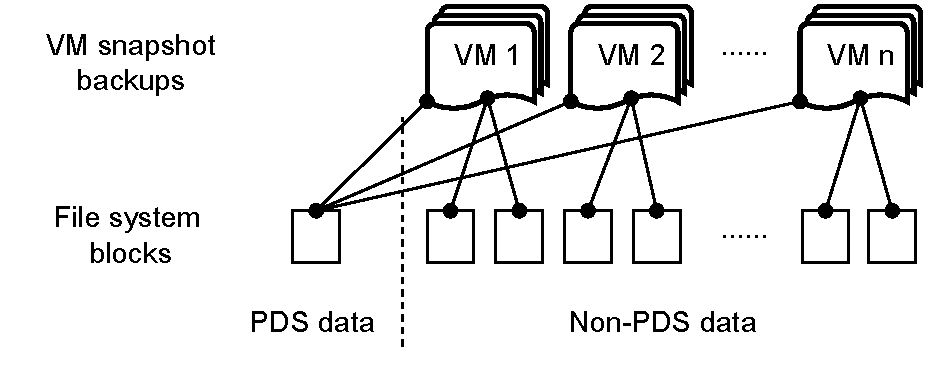
\includegraphics[width=2.9in]{images/share_vc}
        \label{fig:share_vc}
    }
    \\
    \subfigure[Sharing of file system blocks under VO]
    {
        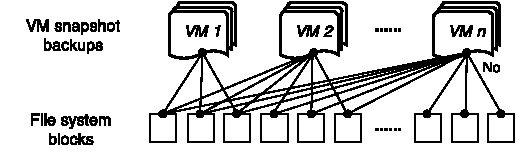
\includegraphics[width=2.9in]{images/share_vo}
        \label{fig:share_vo}
    }
    \caption{Bipartite association of VMs and file blocks. }
    \label{fig:share}
\end{figure}

%We analyze the impact of the above VM centric design on fault isolation and compare it
%with a VM oblivious design.
%Let $r$ be the replication degree of standard file blocks in the underlying backup storage. 
%$r=3$ is a typical setting in distributed file systems~\cite{googlefs03,hdfs10}.
%Let $r_c$ be the replication degree of file blocks for PDS. 
%The replication degree of the backup storage 
%is $r$ for regular file system blocks and 
%Since $\sigma$ is small (e.g.  2\% in our experiments),  
%the impact of replication on storage increase is very small even 
%when choosing  $r_c/r$ ratio as 2 or 3. 


%In the VC approach, a special replication degree $r_c$ is used for PDS data where $r_c>r$. 
%The storage cost for VO with full deduplication is $c_u *r$ and for VC, it is
%$ k*r_c  + (c-E(c-c_u))*r$. Thus The storage cost ratio of $VC$ over $VO$ is 
%\[
%\sigma \frac{r_c}{r} + \frac{c-e(c-c_u)}{c_u}.
%\]
%Since $\sigma$ is small (it is 2\% in our experiments),  
%term $\sigma \frac{r_c}{r}$ is small in the above expression.  
%Thus the impact on storage increase is very small even when we choose a large $r_c/r$ ratio. 
%For example, $r_c/r=2$ or 3. 

Now we  analyze  the impact of losing $d$ physical machines 
to the VM centric and oblivious approaches.  
There are two impacts to VC. 
1) Some PDS fingerprint lookup services do not respond.  As  a result, some duplicates
are not detected and deduplication efficiency suffers, but the overall systems can still
function well and fault tolerance is not affected.  As discussed in Section ~\ref{sect:architecture}, 
PDS index is distributed
among all machines in our implementation and thus a percentage of failed nodes
causes an increase in missed duplicates proportionally.
2) Some storage nodes do not  respond and file blocks on those machines are lost. The availability of
VM snapshots is affected and we analyze this impact as follows.


%A large $r_c/r$ ratio can have a positive impact on full availability of VM snapshot blocks.
%We use an FSB rather than a deduplication
%data chunk as our unit of failure because the DFS keeps
%file system blocks as its base unit of storage.
To compute the full availability of all snapshots of a VM, we estimate
the number of file system blocks per VM and the probability of losing a snapshot file system 
block of a VM in each approach as follows.
Parameters used in our analysis below are defined in Table~\ref{tab:symbol}. 
%As illustrated in Figure~\ref{fig:share},
%we build a bipartite graph representing the association from unique file system blocks
%to their corresponding VMs in each approach. An association edge is  drawn  from an FSB to a VM 
%if this block is used by the VM. 

As illustrated in Figure~\ref{fig:share}, we build a bipartite graph representing the
association from unique file system blocks to their corresponding VMs in two 
approaches. 
%We use a file system block rather than data chunk as our unit of failure
%because the underlying file system keeps file system blocks as its base unit of storage, and in
%the case of 64MB file system blocks  and 4KB chunks, there are 16K chunks per file block. For VM centric,
%we assign extra replication to the PDS blocks, while for VM oblivious, the replication
%degree is fixed.
For VC, each VM has an average number $N_1$ of non-PDS file system blocks
and  has  an average of  $N_2$ PDS file system blocks. 
Each non-PDS block is associated with only one VM.
% and  we denote that PDS blocks are shared by an average of $V_c$ VMs. 
Then by counting outgoing edges from VMs in Figure~\ref{fig:share}(a), we get:
\[
n* N_1   = \mbox{ Number of non-PDS file system blocks in VC.} 
\]

For VO, 
%each VM has an average of $N_o$ file system blocks
%and let $V_o$ be the average number of VMs shared by each file block.
by counting outgoing edges from VMs in Figure~\ref{fig:share}(b) with parameters defined in
Table~\ref{tab:symbol}: 
\[
n *N_o   =  V_o *\mbox{ Number of file system blocks in VO.} 
\]

Since we choose 2-4\% of unique chunks for PDS
and Section~\ref{sect:evaldedup} 
shows that the deduplication efficiency of VC is very close to that of VO,
the number of non-PDS file blocks in VC is fairly close to the number of file blocks in VO.
Then
\[
\frac{N_o}{N_1} \approx  V_o.
\]
%Thus $N_o >> N_1$.

Figure~\ref{fig:vm-links} shows $N_1$, $N_2$, and $N_o$ values of 105 VMs from a  test dataset 
discussed in Section~\ref{sect:evaluation} when increasing the number of VMs.  
%the average number of file system blocks for each VM in VC and in VO
$N_1$ is much smaller than $N_o$ as the formula shows above. 

%In fact, $N_1 +N_2 < N_o$. 
%This is likely because the PDS FSBs tightly pack data used by many VMs, 
%which decreases the overall number of FSBs required to backup a VM.
%Note that  if  the backup for multiple VMs were conducted concurrently, there could be many more
%VMs sharing each file block on average in VO. 

%Therefore, even when there is a loss of a PDS block, the VC approach tolerates the fault better.


\begin{figure}[htbp]
  \centering
	\begin{tikzpicture}
		\begin{axis}[
		%title={VO VM links},
                width=\linewidth,
                height=0.6\linewidth,
		xlabel={Number of VMs},
		ylabel={file system blocks},
                xmin=0,
                ymin=0,
                xmax=106,
		%extra y ticks={4.5,5.5,6.5} %to show extra ticks
		%legend pos=north east,
                legend style={
                    at={(1,0.825)},
                    anchor=north east
                },
                %legend columns=3
		]
                \addplot[blue,mark=none] table[x=VMs,y=N_O] {figures/vm_links_all.txt};
                %\addplot[red,dotted,mark=none] table[x=VMs,y expr=\thisrow{N_1}+\thisrow{N_2}] {figures/vm_links_all.txt};
                \addplot[red,dashdotted] table[x=VMs,y=N_1] {figures/vm_links_all.txt};
                \addplot[red,densely dashed,mark=none] table[x=VMs,y=N_2] {figures/vm_links_all.txt};
                \legend{$N_o$,
                    %$N_1+N_2$,
                    $N_1$,
                    $N_2$};
		\end{axis}
	\end{tikzpicture}
  \caption{Measured average number of 64MB file system blocks used by a single VM in
VC and VO. }
  \label{fig:vm-links}
\end{figure}

%The full snapshot availability of a VM is estimated as follows with parameters $N_1$ and
% $N_2$ for VC and $N_o$ for VO.
Given $d$ failed physical machines and $r$ replicas for each file block,
%normal data replication degree $r$, PDS data replication degree $r_c$, 
the availability of a file block is the probability that  
all of its replicas do not appear in any group of $d$ failed machines among the total of $p$ machines. 
Namely, 
\[
A(r) = 1-\binom{d}{r}/ \binom{p}{r}. 
\]
Then the availability of one VM's snapshot data under VO approach is the probability that
 all its file blocks  are unaffected during the system failure:
%\begin{equation}
%\label{eq:VO}
%(1-\frac{ \binom{d}{r}} { \binom{p}{r} })^{N_o}. 
\[
A(r)^{N_o}. 
\]
%\end{equation}

For VC, there are two cases: $r \le d<r_c$ and $r_c \leq d$.  

\noindent $r \le d<r_c$:  In this case there is no PDS data loss and we need to look at the non-PDS data loss. 
The full snapshot availability of a VM is: 
%\begin{equation}
%\label{eq:VC1}
%(1-\frac{\binom{d}{r}} { \binom{p}{r} })^{N_1}.
\[
A(r)^{N_1}.
\]
%\end{equation}
Since $N_1$ is typically much smaller than $N_o$, 
the VC approach has a higher availability of VM snapshots than VO in this case.
%In the evaluation discussed in Section~\ref{sect:evaldedup}, 
%We have considered a worst case scenario where
%every PDS FSB is shared by all VMs in the VC approach, which leads a large $N_2$ value. 
%Even with $N_2$ being much higher than $N_o$ (as discussed below),
%the availability of VC snapshots is much higher than VO.

\noindent $r_c \leq d$: Both non-PDS and PDS file system blocks in VC can have a loss.
The full snapshot availability of  a VM in the VC approach is
%\begin{equation}
%\label{eq:VC2}
% (1-\frac{ \binom{d}{r}} { \binom{p}{r} })^{N_1} 
% *
% (1-\frac{ \binom{d}{r_c}} { \binom{p}{r_c} })^{N_2}.
\[
A(r)^{N_1} * A(r_c)^{N_2}.
\]
That is still smaller than that of $V_O$ based on the observations of our data. There are two reasons for this:  
1) $N_1$ is much smaller than $N_o$ and we are observing that $N_1+N_2<N_o$. 
2)  $A(r) < A(r_c)$ because $r < r_c$.  
Table~\ref{tab:fsb-availability} lists the $A(r)$ values with
%that the availability of an individual file system block
different replication degrees, to demonstrate the gap between  $A(r)$ and  $A(r_c)$.
%\end{equation}
%comparing  Formula~\ref{eq:VO} and~\ref{eq:VC}. 
%In the evaluation discussed in Section~\ref{sect:evaldedup},
%We have considered a worst case scenario that
%every PDS FSB is shared by all VMs in the VC approach, which leads to a large $N_2$ value. 
%Even with that, the availability of VC snapshots is still much higher than VO and  

% $1-\frac{ \binom{d}{r}} { \binom{p}{r} } < 1-\frac{ \binom{d}{r_c}} { \binom{p}{r_c} }$

\comments{
\begin{figure}[htbp]
  \centering
    \begin{tikzpicture}
            \begin{axis}[
                width=\linewidth,
                height=0.6\linewidth,
            %title={FSB Availability},
            cycle list name=mline,
            xlabel={Number of Machines Failed},
            ylabel={Availability of Single FSB (\%)},
            %extra y ticks={99.9}, %to add extra ticks
            mark options=solid,
            legend pos=south west,
            %legend columns=2,
            %legend style={
            %    at={(0.5,-0.2)},
            %anchor=north}
            ]
            \addplot table[x=NodesFailed,y=Availability5] {figures/fsb_availability.txt};
            \addplot table[x=NodesFailed,y=Availability4] {figures/fsb_availability.txt};
            \addplot table[x=NodesFailed,y=Availability3] {figures/fsb_availability.txt};
            \legend{$R=5$,$R=4$,$R=3$};
            \end{axis}
    \end{tikzpicture}
    \caption{Availability of a file system block in a 100 machine cluster with different replication 
and failure settings.THIS PLOT WILL BE REPLACED BY TABLE}
  \label{fig:fsb-availability}
\end{figure}
}

\begin{table}
  \centering
    \footnotesize
    \tabcolsep=0.11cm
    \comments{%table data is obsolete, now uses pgfplotstable
        \begin{tabular}{|l|l|l|l|}
        \hline
        \multirow{2}{*}{Failures ($d$)}   & \multicolumn{3}{c|}{$A(r_c)\times 100\%$} \\
                                    %\cline{2-4}
                                    & $r_c=3$ & $r_c=6$ & $r_c=9$ \\
        \hline
        3 & 99.9994 & 100 & 100\\
        5 & 99.9939 & 100 & 100\\
        10 & 99.9258 & 99.9999 & 99.9999 \\
        20 & 99.2950 & 99.9967 & 99.9999 \\
        \hline
    \end{tabular}
    }
    \pgfplotstabletypeset[
        columns={NodesFailed,Availability3,Availability6,Availability9},
        columns/NodesFailed/.style={
            column name={\multirow{2}{*}{Failures ($d$)}}
        },
        columns/Availability3/.style={
            column name={\multicolumn{3}{c|}{$A(r_c) \times 100\%$}\\&$r_c=3$},
            fixed, precision=9
        },
        columns/Availability6/.style={
            column name={$r_c=6$},
            fixed, precision=9},
        columns/Availability9/.style={
            column name={$r_c=9$},
            fixed, precision=9},
        every head row/.style={
            before row={\hline},
            after row={\hline},
        },
        every last row/.style={after row=\hline},
        column type/.add={}{|},
        every first column/.style={column type/.add={|}{}},
    ]{figures/fsb_availability.txt}
    \caption{$A(r_c)$ values in a cluster with p=100 nodes.}
    \label{tab:fsb-availability}
\end{table}


\comments{
\subsection{Impact on Deduplication Efficiency}
Choosing the value $k$ for the most popular chunks affects the deduplication efficiency.
We analyze this impact based on the characteristics  of the VM snapshot traces
studied from  application datasets.
A previous study shows that the popularity of data chunks after local deduplication follows 
a Zipf-like distribution\cite{Breslau1999a} and its
exponent $\alpha$ is ranged between 0.65  and  0.7~\cite{WeiZhangIEEE}. 
Figure~\ref{fig:Datazipf} illustrates the Zipf-like distribution of chunk popularity.
The parameters we will use in our analysis below are defined in
Table~\ref{tab:symbol}. 

%Table~\ref{tab:symbol} defines paramters $c$, $c_u$, $f_i$, and $\delta$ used below.
%let $c$ be the total number of data chunks. 
%$c_u$ be the total number of fingerprints 
%in the global index after complete deduplication, and
%$f_i$ be the frequency for the $i$th most popular fingerprint. 
By Zipf-like distribution, $f_i = {f_1}/{i^\alpha}.$
The total number of chunks in our backup storage which
has local duplicates excluded is $c (1-\delta)$, this can be represented
as the sum of each unique fingerprint times its frequency:
%Since $ \sum_{i=1}^{c_u}f_i = c (1-\delta)$,
\[
f_1 \sum_{i=1}^{c_u}\frac{1}{i^\alpha} = c (1-\delta).
\]
Given $\alpha <1$, $f_1$ can be approximated with integration:
%\begin{equation}
\[
f_1=\frac{c(1-\alpha)(1-\delta)}{c_u^{1-\alpha}}.
\]
%\end{equation}

Thus putting the $k$ most popular fingerprints into PDS index can remove the following number of chunks during global 
deduplication:
\[
f_1 \sum_{i=1}^{k}\frac{1}{i^\alpha} \approx  
f_1 \int_{1}^{k}\frac{1}{x^\alpha} dx  \approx  f_1\frac{  k^{1-\alpha}} {1-\alpha}
=c(1-\delta) \sigma^{1-\alpha}.
\]

Deduplication efficiency of the VC approach using top $k$ popular chunks
is the percentage of duplicates that can be detected:  
\begin{equation}
\label{eq:dedupeff}
%\begin{split}
%e_k &= 
E_c=\frac{ c\delta + c(1-\delta) \sigma^{1-\alpha}}
{c  - c_u }.\\
%\end{split}
\end{equation}

% After the global deduplication, the number of remaining chunks is:
% \[
% c-E(c-c_u)
% \] 

We store the PDS index using a distributed shared memory hash table such as Memcached
and allocate a fixed percentage of memory space per physical machine for top $k$ popular items.
As the number of physical machines ($p$) increases,
the entire cloud cluster can host more VMs; however,  ratio $\sigma$ which is $k/c_u$ remains
a constant because each physical machine on average still hosts a fixed constant number of 
VMs. Then the overall deduplication efficiency of VC defined in Formula~\ref{eq:dedupeff}
remains constant.
Thus the deduplication efficiency is stable  as $p$ increases as long as $\sigma$  is a constant.


\begin{figure}[htbp]
  \centering
    \begin{tikzpicture}
            \begin{axis}[
            %title={PDS Coverage},
            width=\linewidth,
            height=0.6\linewidth,
            cycle multi list={
                mline\nextlist
                [3 of]mmark*\nextlist
            },
            %cycle list name=mcolor,
            xlabel={Total num. chunks stored (in billions)},
            ylabel={PDS Coverage (\%)},
            %extra y ticks={4.5,5.5,6.5} %to add extra ticks
            mark options=solid,
            %legend pos=outer north east,
            legend columns=2,
            legend style={
                at={(0.5,-0.30)},
            anchor=north},
            ]
            \addplot table[x expr=\thisrow{InputChunks}/1000000000,y=A1] {figures/cds_coverage.txt};
            \addplot table[x expr=\thisrow{InputChunks}/1000000000,y=A2] {figures/cds_coverage.txt};
            \addplot table[x expr=\thisrow{InputChunks}/1000000000,y=A4] {figures/cds_coverage.txt};
            \addplot table[x expr=\thisrow{InputChunks}/1000000000,y=T1] {figures/cds_coverage.txt};
            \addplot table[x expr=\thisrow{InputChunks}/1000000000,y=T2] {figures/cds_coverage.txt};
            \addplot table[x expr=\thisrow{InputChunks}/1000000000,y=T4] {figures/cds_coverage.txt};
            \legend{Measured ($\sigma=1\%$),Measured ($\sigma=2\%$),Measured ($\sigma=4\%$),Predicted ($\sigma=1\%$),Predicted ($\sigma=2\%$),Predicted ($\sigma=4\%$)};
            \end{axis}
    \end{tikzpicture}
  \caption{Predicted vs. actual PDS coverage as data size increases.}
  \label{fig:cds-coverage}
\end{figure}
Ratio $\sigma^{1-\alpha}$ represents the percentage of the remaining
chunks detected as duplicates in global deduplication due to PDS.
We call this PDS coverage.
Figure~\ref{fig:cds-coverage} shows predicted PDS coverage using $\sigma^{1-\alpha}$ when $\alpha$ is fixed at
0.65 and measured PDS coverage in our test dataset.
$\sigma=2\%$ represents memory usage of approximately 100MB memory per machine for the PDS.
While the predicted value remains flat, measured PDS coverage increases as more VMs are involved.
This is because the actual $\alpha$ value increases with the data size.
%Then  PDS coverage PDS increases as more VMs are involved.
}
